\documentclass[letterpaper, 12pt]{article}
\usepackage[margin=1in]{geometry}
\usepackage{graphicx}
\usepackage{listings}
\usepackage{color}
\graphicspath{{images/}{../Template/images/}}
\lstset{language=C,basicstyle=\ttfamily,keywordstyle=\color{blue}\ttfamily,stringstyle=\color{red}\ttfamily,commentstyle=\color{green}\ttfamily,morecomment=[l][\color{magenta}]{\#},tabsize=2,showstringspaces=false,frame=single}

\newcommand{\hwnumber}{Lab 7}
\newcommand{\duedate}{November 14th, 2015}

\newcommand{\capper}{\begin{flushright}Aviles, Jean-Ralph \\ EEL3744 \\ Section 1539 \\ \duedate{} \\ \hwnumber{}\end{flushright}}

\begin{document}
\capper{}
\section*{Questions}
\begin{enumerate}
  \item Draw a 15 kHz square wave with 66\% duty cycle.
    \begin{center}
      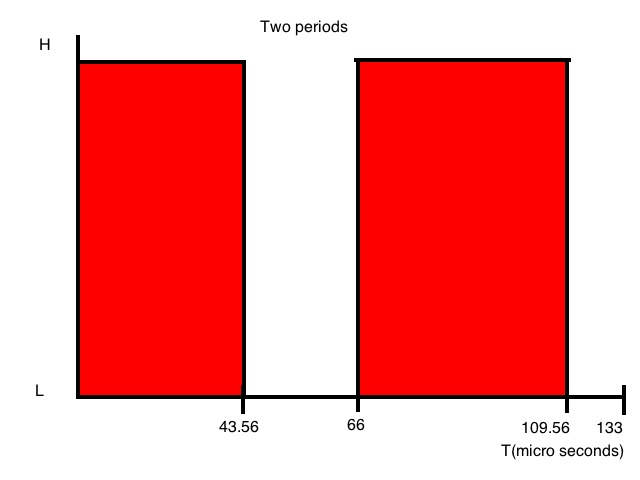
\includegraphics[scale=0.6]{square_wave}
    \end{center}
  \item For part A, what is the limiting factor for the precision of your frequency generation? Can your XMEGA generate some frequency ranges with higher precisions than other frequency ranges? Explain. \\
    The limiting factor for our frequency generation is the value of CCA. At its lowest, CCA can be 0. Using the equation in the appendix
    the higheset frequency we could get is 1Mhz, which is a period of $1\mu s$. I don't think the Xmega an generate more precise signals. We're getting
    too close to have enough clock cycles to do anything else.
  \item How does the prescaler affect the way the TC system counts per clock cycle? Where are the counts stored? \\
    The prescaler sets how many clock ticks count for one TC count. The counts that make it through are stored
    in a device called a base counter.
  \item Describe the difference(s) between the TC’s Frequency Generation mode and its Single/Dual Slope PWM modes. Which mode(s) can be used to emulate the other(s)? How could you make a sine wave or other waveform using your XMEGA by using the timer system? Do you need to add any extra hardware? How can you produce these waveforms without extra hardware? \\
    The Frequency generation mode does a lot of the hard work for you, reseting the counter at a certain value, getting the timing right, while the PWM modes require a bit more intervention by the user. The PWM mode can be used to emulate the Frequency mode, but not the other way around as you can do things like change the duty cycle with the PWM mode.
    You can make a sine wave with a PWM system by slowly increasing the duty cycle of a signal over time to get a higher average value. You don't need any extra hardware you just need a quite involved software program to do all the math and duty cycle changes.
\end{enumerate}
\section*{Problems Encountered}
None this time. It went smoothly. Mainly because I used avr-gcc and never
booted into my Windows VM.
\section*{Future Work/Applications}
We can use the frequency generation capabilities of the Xmega to control
other speakers to generate music or use PWM to control servos and motors.
\section*{Appendix}
\subsection*{Part A}
\begin{itemize}
  \item I chose to use PORTE\_PIN3 as the output port for my speaker.
  \item Since I'm using the Frequency Generation mode for the TC. CCA
    must be set to the correct value for the desired frequency. For a
    given frequency, we can calulate the CCA vaue required with by
    solving the formula given to us in the manual on page 172\ldots
    \[ F\textsubscript{FRQ} = \frac{f\textsubscript{clk\textsubscript{per}}}{2N(CCA+1)} \Rightarrow CCA = \frac{f\textsubscript{clk\textsubscript{per}}}{2NF\textsubscript{FRQ}} - 1 \]
    Where $F_{FRQ}$ is the desired frequency, CCA is the value of the CCA register, $F_{clk_{per}}$ is the system clock rate, and N is the clock prescaler.
      \begin{itemize}
          \item For PartA to generate a 1760Hz signal, we would have to put a value of
            \[ CCA = \frac{2*10^{6}}{2*1760} - 1 \Rightarrow CCA = 567 \] into the CCA register.
      \end{itemize}
    \item Wiring diagram for the speaker\ldots
      \begin{center}
        \includegraphics[scale=0.6]{speaker}
      \end{center}
    \item Generated 1760Hz signal viewed on the DAD.
      \begin{center}
        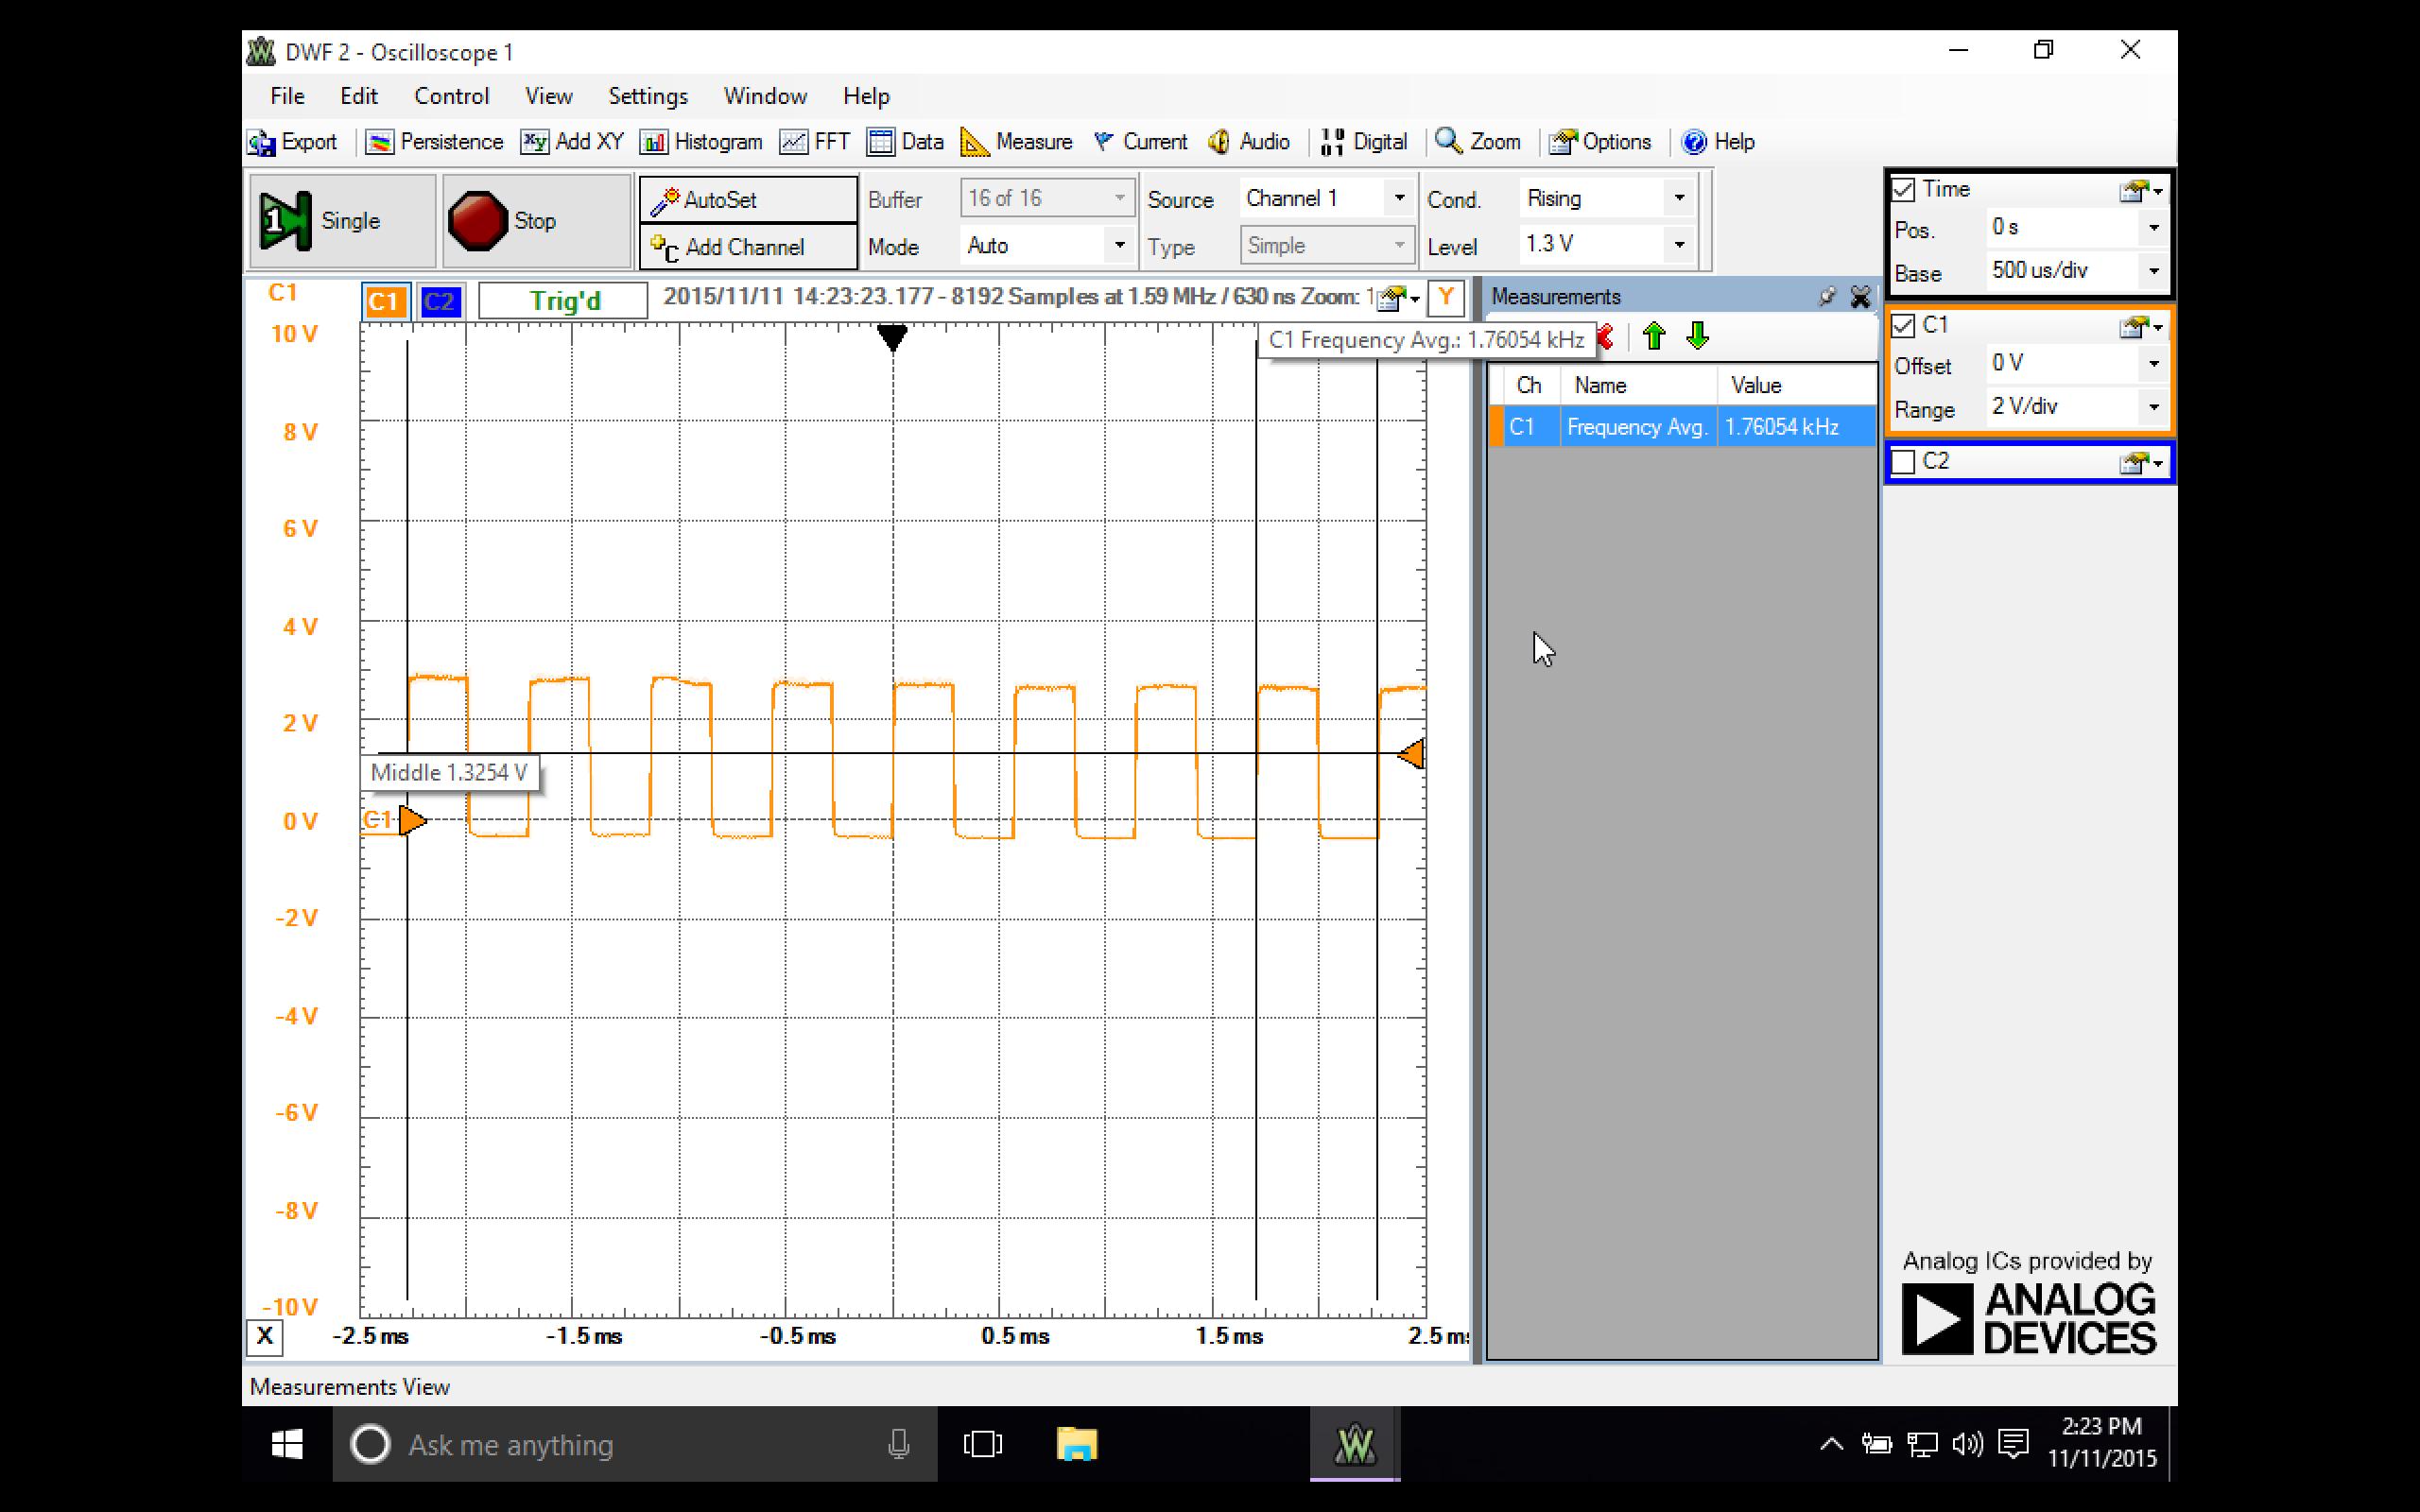
\includegraphics[scale=0.3]{parta_dad.png}
      \end{center}
\end{itemize}
\subsection*{Part B}
\begin{itemize}
  \item CCA Values for Various Notes
    \begin{center}
      \begin{tabular}{| c | c | c |}
        \hline
        Note & Frequency & CCA Value \\
        \hline\hline
        C\textsubscript{5}\# & 523.25 & 1910.132 \\
        \hline
				C\textsubscript{5}\# & 554.37 & 1802.849415 \\
        \hline
				D\textsubscript{5} & 587.33 & 1701.620333 \\
        \hline
				D\textsubscript{5}\# & 622.25 & 1606.071113 \\
        \hline
				E\textsubscript{5} & 659.25 & 1515.875237 \\
        \hline
				F\textsubscript{5} & 698.46 & 1430.721215 \\
        \hline
				F\textsubscript{5}\# & 739.99 & 1350.369613 \\
        \hline
				G\textsubscript{5} & 783.99 & 1274.526474 \\
        \hline
				G\textsubscript{5}\# & 830.61 & 1202.934458 \\
        \hline
				A\textsubscript{5} & 880 & 1135.363636 \\
        \hline
				A\textsubscript{5}\# & 932.33 & 1071.581597 \\
        \hline
				B\textsubscript{5} & 987.77 & 1011.381425 \\
        \hline
      \end{tabular}
      \begin{tabular}{| c | c | c |}
        \hline
        Note & Frequency & CCA Value \\
        \hline\hline
				C\textsubscript{6} & 1046.5 & 954.566173 \\
				\hline
				C\textsubscript{6}\# & 1108.73 & 900.9328421 \\
				\hline
				D\textsubscript{6} & 1174.66 & 850.3101663 \\
				\hline
				D\textsubscript{6}\# & 1244.51 & 802.5290998 \\
				\hline
				E\textsubscript{6} & 1318.51 & 757.4318663 \\
				\hline
				F\textsubscript{6} & 1396.91 & 714.8657322 \\
				\hline
				F\textsubscript{6}\# & 1479.98 & 674.6848066 \\
				\hline
				G\textsubscript{6} & 1567.98 & 636.7632368 \\
				\hline
				G\textsubscript{6}\# & 1661.22 & 600.9672289 \\
				\hline
				A\textsubscript{6} & 1760 & 567.1818182 \\
				\hline
				A\textsubscript{6}\# & 1864.66 & 535.2907983 \\
				\hline
				B\textsubscript{6} & 1975.53 & 505.1932747 \\
				\hline
      \end{tabular}
    \end{center}
\end{itemize}
\section*{Pseudocode/Flowcharts}
\subsection*{Part A}
\lstinputlisting{code/Lab7_PartA.ps}
\subsection*{Part B}
\lstinputlisting{code/Lab7_PartA.ps}
\subsection*{Headers}
\subsubsection*{Helpers}
\lstinputlisting{code/helpers.ps}
\subsubsection*{Keypad}
\lstinputlisting{code/keypad.ps}
\subsubsection*{Lcd}
\lstinputlisting{code/lcd.ps}
\subsubsection*{Speaker}
\lstinputlisting{code/speaker.ps}
\section*{Programs}
\subsection*{Part A}
\lstinputlisting{code/Lab7_PartA.c}
\subsection*{Part B}
\lstinputlisting{code/Lab7_PartA.c}
\subsection*{Headers}
\subsubsection*{Helpers}
\lstinputlisting{code/helpers.h}
\subsubsection*{Keypad}
\lstinputlisting{code/keypad.h}
\subsubsection*{Lcd}
\lstinputlisting{code/lcd.h}
\subsubsection*{Speaker}
\lstinputlisting{code/speaker.h}
\end{document}
